\documentclass[a4paper,12pt]{report}

\usepackage{graphicx}
\usepackage[utf8]{inputenc}
\usepackage{hyperref}
\usepackage[left=2cm,right=2cm,top=2cm,bottom=2cm]{geometry}

\usepackage{lipsum}% http://ctan.org/pkg/lipsum
\usepackage{titletoc}% http://ctan.org/pkg/titletoc
\titlecontents*{chapter}% <section-type>
  [0pt]% <left>
  {}% <above-code>
  {\bfseries\chaptername\ \thecontentslabel\quad}% <numbered-entry-format>
  {}% <numberless-entry-format>
  {\bfseries\hfill\contentspage}% <filler-page-format>



\begin{document}

\graphicspath{{images/}}


\title{2nd Report \\ \textbf{Face Detection Techniques And Algorithms}}
	\author{----------------------------- \\   \\  \\   \\   \\   \\  \\   \\   \\   \\   \\ \textbf{Supervised by:}\\ Prof. Oussama El Issati\\ \textbf{Prepared by:} \\ Ait Said Noureddine \\ Ennouali Mohamed Amine}
	\maketitle



\maketitle

\tableofcontents


%\begin{abstract}


%\end{abstract}

\chapter{Face detection techniques and algorithms}
  \section{Introduction}
    Object detection is a computer technology related to computer vision and image processing that deals with detecting instances of semantic objects of a certain class (such as humans, buildings, or cars) in digital images and videos. Well-researched domains of object detection include face detection and pedestrian detection. Object detection has applications in many areas of computer vision, including image retrieval and video surveillance. \par
    Object detection algorithms are used in face detection and face recognition. It is also used in tracking objects, for example tracking a ball during a football match, tracking movement of a cricket bat, tracking a person in a video.\par
    The concept is that every object class has its own special features that helps in classifying the class – for example all circles are round. Object class detection uses these special features. For example, when looking for circles, objects that are at a particular distance from a point (i.e. the center) are sought. Similarly, when looking for squares, objects that are perpendicular at corners and have equal side lengths are needed. A similar approach is used for face identification where eyes, nose, and lips can be found and features like skin color and distance between eyes can be found\cite{wiki_link}.\par

\section{Face detection and tracking algorithms}
    Cascading is an ensemble learning based on the concatenation of several Classifiers, using all information collected from the output from a given classifier as additional information for the next classifier in the cascade. Cascading is a multistage system.\par
    Cascading classifiers are trained with several hundred ``\emph{positive}'' sample views of a particular object and arbitrary ``\emph{negative}'' images of the same size. \par
    After the classifier is trained it can be applied to a region of an image and detect the object in question. To search for the object in the entire frame, the search window can be moved across the image and check every location for the classifier. This process is most commonly used in image processing for object detection and tracking, primarily facial detection and recognition.\par

\subsection{Cascade classification based algorithm: Viola and Jones}
   The first cascading classifier is the face detector of \emph{Viola and Jones (2001)}. The requirement was that the classifier be fast in order to be implemented on low CPU systems, such as cameras and phones\cite{wiki_link}.\par
  \begin{figure}[h]
    \centering
    \caption{\label{cascade_concept} Concept of cascade classification\cite{haar_lbp_hog_comp_pdf}}
    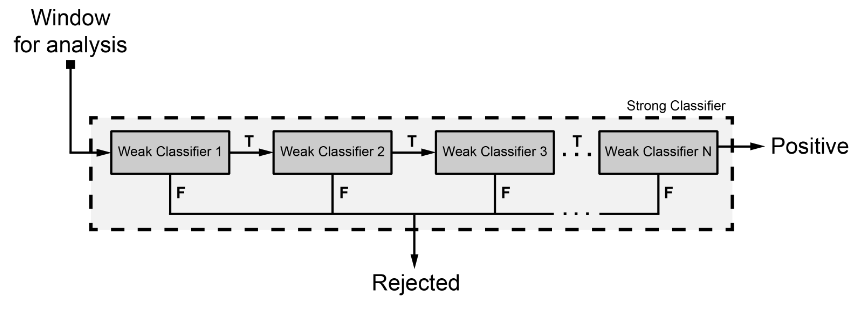
\includegraphics[scale=0.55]{cascade_concept.png}
  \end{figure}

\subsubsection{Characteristics of the algorithm}

  \begin{itemize}
      \item \textbf{Robust:} the algorithm has a very high detection rate (true-positive rate) and very low false-positive rate\footnotemark.
      \item \textbf{Real Time:}  At least 2 frames per second are processed thus making it a quick and an efficient algorithm. The algorithm comprises of four stages: 


      \begin{enumerate}
	\item Haar Features Selection 
	\item Creating Integral Image
	\item Adaboost Training Algorithm 
	\item Cascade Classifiers 
      \end{enumerate}

  \end{itemize}

\subsubsection{HAAR Features}
      Haar-like features are digital image features used in object detection\cite{viola_jones}. Haar features are similar to convolution 
      kernels which are used to detect the presence of a feature in the given image. 

%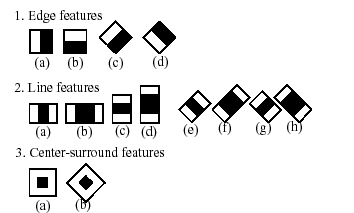
\includegraphics{haar_features.jpg}

      \begin{figure}[h]
	\centering
	\caption{\label{haar_feature} Haar features applied to detect faces\cite{opencv_website}.}
	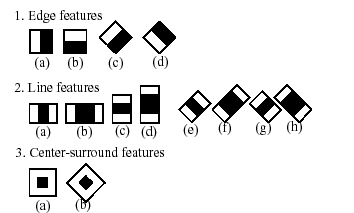
\includegraphics[scale=0.62]{haar_features.png}
	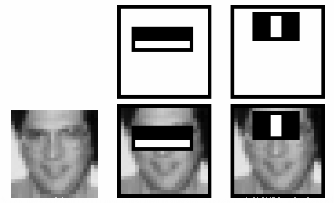
\includegraphics[scale=0.62]{haar_applied.png}
      \end{figure}

      A Haar-like feature considers adjacent rectangular regions at a specific location in a detection window, sums up the pixel intensities in each region and calculates the difference between these sums. \cite{opencv_website}\par
      There is a huge number of possible sizes and locations of each kernel. For example using a 24x24 window results over 160000 features. For each feature calculation, we need to find sum of pixels under white and black rectangles. To solve this, they introduced the integral images to simplify calculation of sum of pixels\cite{sonia_pdf}.

%Dans la figure~\ref{haar_feature} page~\pageref{haar_feature}

\subsubsection{Integral image}
      he  algorithm  introduces  the 
      concept of integral image to find the sum of all the pixels under a rectangle with just 4 corner values instead of 
      summing  up all the values.

\subsubsection{Adaboost}
      Since not all the features are relevant, we have to select only the best features using Adaboost. Which is  a  machine  learning  algorithm  which  helps  in  finding  only  the  best  features  among  all  the 
      160000+ features. After  these  features  are  found,  a  weighted  combination  of  all  these  features  is  used  in 
      evaluating  and  deciding  if  any  given  window  (24x24)  has  a  face  or  not.  Each  of  the  selected  feature  is 
      considered to be included if they can at least perform better than random guessing. The little classifiers are called ``weak classifiers'', Adaboost  constructs  a  strong  classifier  as  a  linear 
      combination of these weak classifiers.

\subsubsection{HAAR classifier generating}
      The process of generating a classifier includes two stages: the training and the detection stage. The detection stage using either HAAR or LBP based models. The library \textbf{OpenCV} comes with preprogramed applications that we can use to generate a classifier in $.xml$ file, this file contains all the features that will be used to look for faces in future applications, OpenCV comes also with pre-generated $.xml$ files ready to use.

      \begin{figure}[h]
	\centering
	\caption{\label{haar_stage_vis} The process of classifier generation using OpenCV.}
	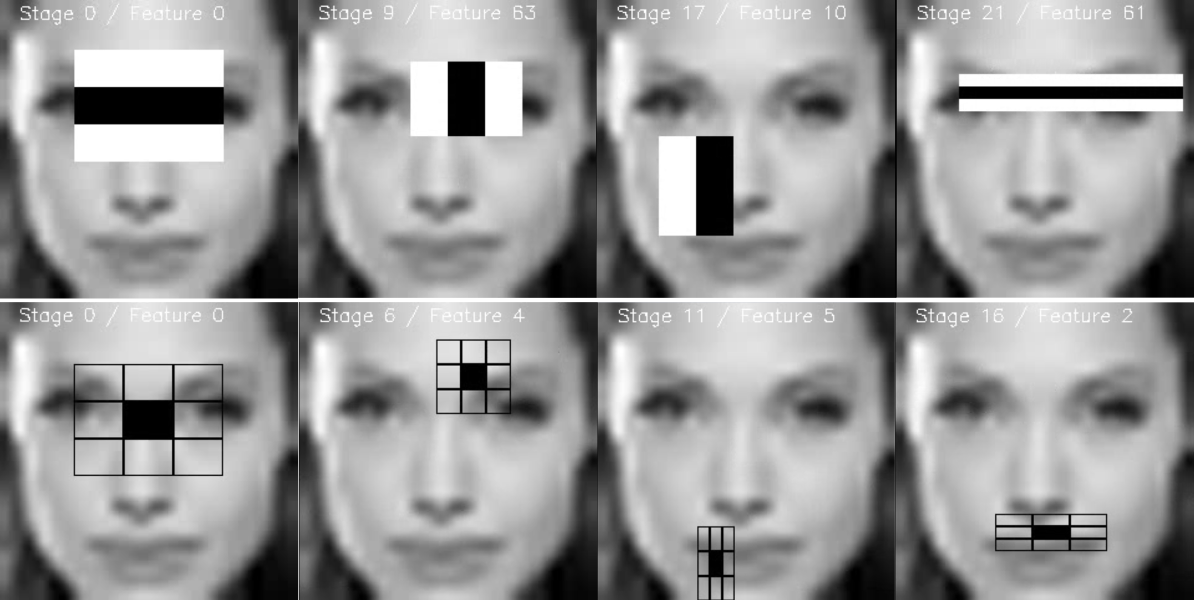
\includegraphics[scale=0.5]{haar_stage_vis.png}
      \end{figure}

\subsubsection{Advantages}

      \begin{itemize}
      \item Fast features are computed very quickly. 
      \item The features are scaled instead of scaling the image. 
      \item This is a generic detection scheme which can be used to detect other objects like hands, buildings, etc. 
      \end{itemize}

\subsubsection{Disadvantages}

      \begin{itemize}
	\item The detector is effective only in the case of frontal images of the face. 
	\item If the face is turned 45 degrees, it fails to detect the face. 
	\item It is sensitive to lighting conditions.
	\item Due  to  overlapping  sub-windows,  we  might  face  the  problem  of  multiple  objects  being  detected  as face. 
      \end{itemize}

\subsubsection{Results}

      \begin{figure}[h]
	\centering
	\caption{\label{haar_result} Default OpenCV HAAR cascade classifier test.}
	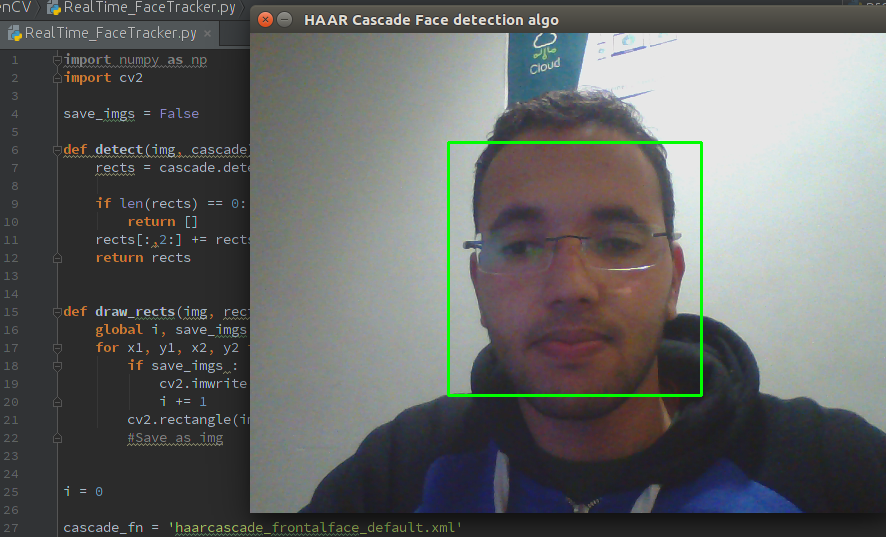
\includegraphics[scale=0.5]{haar_test.png}
      \end{figure}


\subsection{CAMshift Algorithm}
    CAMshift is a tracking algorithm, which is based on MeanShift algorithm, what CAMshift does meanShift in every single frame of a video, and record the results we got by MeanShift. 
    CamShift algorithm includes these three parts\cite{camshift} :
    
      \begin{enumerate}
	\item Back projection 
	\item Applying MeanShift
	\item Tracking
	    
      \end{enumerate}
  
  \subsubsection{Back Projection}
  
  Back projection is a method using the histogram of an image to show up the probabilities of colors that may appear in each pixel.
First we transform the picture space to HSV space which is a cylindric color base (or any space which include an H channel that represent the hue of each pixel, of course, value of hue is between 0 to 180). Secondly, we split the H channel out, as a single grayscale image, and get its histogram, and normalize it. Thirdly, we use “calcBackProject()” function to calculate the back projection of the image.

  \textbf{Example:} 
  
This is an example to explain how we get the back projection.   We transform the picture into HSV space and the second image shows the hue channel. The third image shows its histogram.
We calculate the weight of each color in the whole picture using histogram, and change the value of each pixel to the weight of its color in whole picture, the result of this step is shown in the last image.
  \begin{figure}[h]
    \centering
    %\lefting
    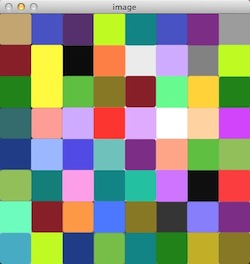
\includegraphics[scale=0.55]{backpro1.jpeg}
     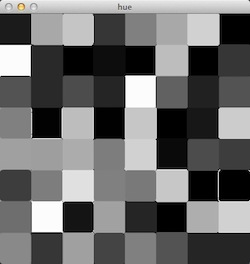
\includegraphics[scale=0.55]{backpro2.jpeg}
     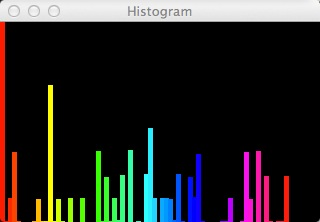
\includegraphics[scale=0.62]{backpro3.jpg}
     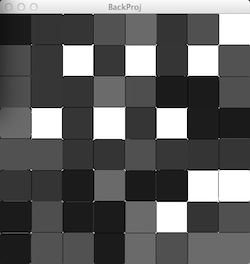
\includegraphics[scale=0.55]{backpro4.jpeg}

  \end{figure}
  
  
  \subsubsection{Applying MeanShift}
  
  MeanShift is an algorithm which finding modes in a set of data samples representing an underlying probability density function, so the whole algorithm is:

      \begin{enumerate}
	\item Initialize the sphere, including the center and radius.
	\item Calculate the current mass center.
	\item Move the sphere’s center to mass center
	\item Rrepeat step b and c, until converge, that is, current mass center after calculate, is the same point with center of sphere.
	    
      \end{enumerate}
  
  \begin{figure}[h]
    \centering
    %\lefting
    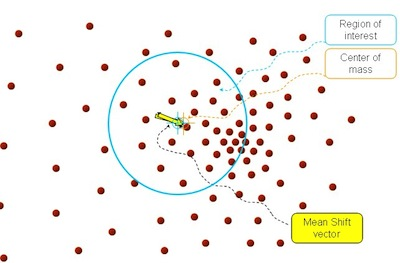
\includegraphics[scale=0.7]{meanshift2.jpg}
    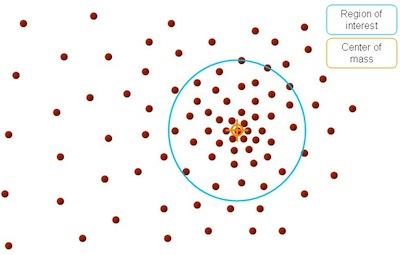
\includegraphics[scale=0.7]{meanshift3.jpg}
    \caption{The meanshift method.}

  \end{figure}
  
    \subsubsection{Track}

    The last step is tracking, if we have a video, or frames captured by our web camera, what we need to do is just use meanShift algorithm to every single frame, and the initial window of each frame is just the output window of the prior frame.
 
  
    \section{Conclusion}
    As a conclusion, CAMshift and HAAR Cascade are two different methods used for detection ; the first one is used for tracking the specified object detected with the second method, so even if there is a permanent movement of the object that we want to detect ,with the collaboration of this two methods the detection will be succeeded.
    
 
    
\chapter{Face recognition methods}  
	\section{Introduction}
	We have developed a near-real-time computer system that can locate and track a subject's head, and then recognize the person by comparing characteristics of the face to those of known individuals. The technology of face recognition has become mature within these few years. Systems using the face recognition, have become true in real life. In this report, we will see a comparative study of the most recent methods of face recognition. One of the approaches is using the eigenfaces method, fisherfaces method, LBPH and SIFT methods. After the implementation of the above methods, we learned the advantages and disadvantages of each approach and the difficulties of their implementation.
	
	\section{The Eigenfaces method}
		Eigenfaces are the name given to a set of eigenvectors when they are used in a computer vision problem of human face recognition. The approach of using eigenfaces for recognition was developed by Sirovich and Kirby (1987) and used by Matthew Turk and Alex Pentland in face classification. The eigenvectors are derived from the covariance matrix of the probability distribution over the high-dimensional vector space of face images.
		  
		\subsection{Individual features}
			
			\begin{itemize}
				\item {Eyes, nose, mouth, head outline}
				\item {Position and size relationships}
			\end{itemize}
			
			\begin{figure}[h]
				\centering
				\caption{\label{face recognation} The Eigenfaces method principal features\cite{haar_lbp_hog_comp_pdf}}
				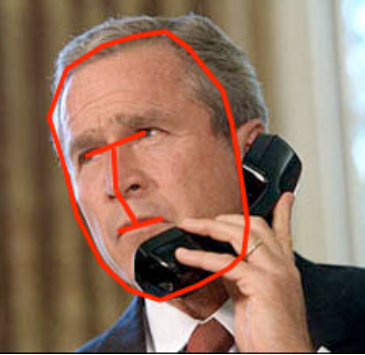
\includegraphics[scale=0.55]{capture0.png}
			\end{figure}
			
		\subsection{Advantages}
			As an appearance-based approach, eigenface recognition method has several advantages:
			\begin{itemize}
				\item {Raw intensity data are used directly for learning and recognition without any significant low-level or mid-level processing.}
				\item {No knowledge of geometry and reflectance of faces is required.}
				\item {Data compression is achieved by the low-dimensional subspace representation.}
				\item {Recognition is simple and efficient compared to other matching approaches.}
			\end{itemize}
			
		\subsection{Disadvantages}
			These advantages reflect the power of appearance-based approach in ease of implementation. However, the experimental results also demonstrate some serious limitations of eigenface representation method for face recognition under different conditions.
			\begin{itemize}
			      \item{very sensitive to scale.}
			      \item{Recognition rate decreases for recognition under varying pose and illumination.}
			      \item{Fragile and complex}
			\end{itemize}
			
			Though the eigenfaces approach is shown to be robust when dealing with expression and glasses, these experiments were made only with frontal views. The problem can be far more difficult when there exists extreme change in pose as well as in expression and disguise. Additionally, all the face images tested in the experiments are taken with a uniform background. However, this condition may not be satisfied in most natural scenes, which will seriously deteriorate the recognition performance. In such cases, a segmentation process has to be considered. 
			
		\subsection{The Eigenface approach}
		\begin{figure}[h]
					\centering
					\caption{\label{face recognation} The Eigenfaces approach \cite{haar_lbp_hog_comp_pdf}}
					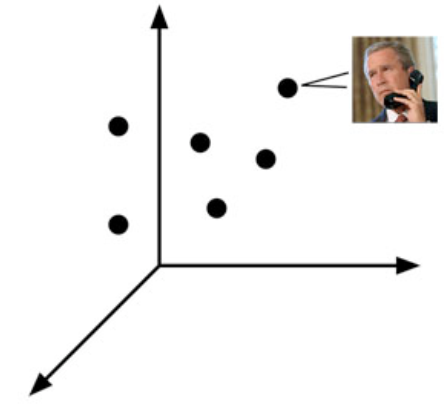
\includegraphics[scale=0.55]{capture1.png}
				\end{figure}
				
				\begin{itemize}
				      \item {Images are points in a vector space.} 
				      \item {We use PCA to reduce dimensionality of the face space.} 
				      \item {Compare projections onto face space to recognize faces.}
				\end{itemize}
				
				
			
	\section{The Fisherfaces method}
				Fisherface Concept-Differing from the Eigenface concept, the fisherface method tries to maximize the ratio of the between-class scatter versus the within-class scatter . The result of this shapes the projections so that the distances between the classes are at a maximum, while the distances between samples of the same class are at a minimum. A possible disadvantage is if the between-class scatter is large, then the within-class scatter might also still be of a relatively large value.
			
				\subsubsection{conclusion}
				Eigenfaces and Fisherfaces take a somewhat holistic approach to face recognition. You treat your data as a vector somewhere in a high-dimensional image space. We all know high-dimensionality is bad, so a lower-dimensional subspace is identified, where (probably) useful information is preserved. The Eigenfaces approach maximizes the total scatter, which can lead to problems if the variance is generated by an external source, because components with a maximum variance over all classes aren’t necessarily useful for classification. So to preserve some discriminative information we applied a Linear Discriminant Analysis and optimized as described in the Fisherfaces method. The Fisherfaces method worked great... at least for the constrained scenario we’ve assumed in our model.
				Now real life isn’t perfect. You simply can’t guarantee perfect light settings in your images or 10 different images of a person. So what if there’s only one image for each person? Our covariance estimates for the subspace may be horribly wrong, so will the recognition. Remember the Eigenfaces method had a 96% recognition rate. How many images do we actually need to get such useful estimates? 
				
				\begin{figure}[h]
					\centering
					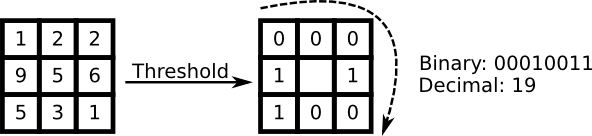
\includegraphics{pic2.png}
				\end{figure}
			
				\subsubsection{The Fisherface approach}
				
				So in order to get good recognition rates you’ll need at least 8(+-1) images for each person and the Fisherfaces method doesn’t really help here. The above experiment is a 10-fold cross validated result carried.
				So some research concentrated on extracting local features from images. The idea is to not look at the whole image as a high-dimensional vector, but describe only local features of an object. The features you extract this way will have a low-dimensionality implicitly. But you’ll soon observe the image representation we are given doesn’t only suffer from illumination variations. Think of things like scale, translation or rotation in images - your local description has to be at least a bit robust against those things. the Local Binary Patterns methodology has its roots in 2D texture analysis. The basic idea of Local Binary Patterns is to summarize the local structure in an image by comparing each pixel with its neighborhood. Take a pixel as center and threshold its neighbors against. If the intensity of the center pixel is greater-equal its neighbor, then denote it with 1 and 0 if not. You’ll end up with a binary number for each pixel, just like 11001111. So with 8 surrounding pixels you’ll end up with 2^8 possible combinations, called Local Binary Patterns or sometimes referred to as LBP codes. For example a LBP operator described in literature used a fixed 3 x 3 neighborhood just like this:
				      
			      \begin{figure}[h]
				      \centering
				      \caption{\label{Face recognition} LBPH principe\cite{haar_lbp_hog_comp_pdf}}
				      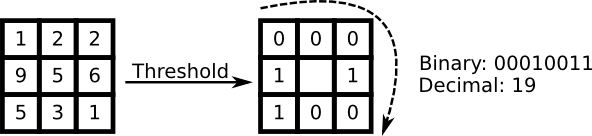
\includegraphics[scale=0.55]{pic2.png}
			      \end{figure}
			      
			      
			      
		\subsection{SIFT Algorithm}
			      
			      \textbf{Scale-invariant feature transform (SIFT)} is an algorithm in computer vision to detect and describe local features in images. The algorithm was patented in the US by the University of British Columbia \cite{uspatent_sift} and published by David Lowe in 1999.\cite{Lowe_David}

			      Applications include object recognition, robotic mapping and navigation, image stitching, 3D modeling, gesture recognition, video tracking, individual identification of wildlife and match moving. \\
			      
			      Due to time limitation, we will not dive deep into this method in this document, we will only present some key notes that distinguish it from the other methods.
			      
			      \subsubsection{Overview}
			      
			      SIFT is simply an algorithm that extracts the key points that distinguish a specific object. This description, extracted from a training image, can then be used to identify the object when attempting to locate the object in a test image containing many other objects.
			      To perform reliable recognition, it is important that the features extracted from the training image be detectable even under changes in image scale, noise and illumination. Such points usually lie on high-contrast regions of the image, such as object edges.
			      The relative positions between these key features in the original scene shouldn't change from one image to another.
			  
			      SIFT detects and uses a very large number of features from the images, which reduces the contribution of the errors caused by these local variations in the average error of all feature matching errors.
			      This technique can robustly identify objects even among clutter and under partial occlusion, because the SIFT feature descriptor is invariant to uniform scaling, orientation, illumination changes, and partially invariant to affine distortion.\cite{uspatent_sift}
			      
			      \subsubsection{How does SIFT work?}
			      SIFT keypoints of objects are first extracted from a set of reference images\cite{Lowe_David} and stored in a database.
			      An object is recognized in a new image by individually comparing each feature from the new image to this database and finding candidate matching features based on Euclidean distance of their feature vectors.
			      From the full set of matches, subsets of keypoints that agree on the object and its location, scale, and orientation in the new image are identified to filter out good matches.
			      The determination of consistent clusters is performed rapidly by using an efficient hash table implementation of the generalized Hough transform. Each cluster of 3 or more features that agree on an object and its pose is then subject to further detailed model verification and subsequently outliers are discarded. Finally the probability that a particular set of features indicates the presence of an object is computed, given the accuracy of fit and number of probable false matches. Object matches that pass all these tests can be identified as correct with high confidence.\cite{Lowe_David_2}
			      
			      \subsubsection{An example of application}
			      
			      
		\subsection{}
			      

\begin{thebibliography}{9}
  \bibitem{wiki_link} 
    \textit{Wikipedia}.\\
    \url{https://en.wikipedia.org/wiki/Object_detection} \\
    \url{https://en.wikipedia.org/wiki/Computer_vision}
    
  \bibitem{viola_jones}
    P. Viola,  M.J. Jones
    \textit{``Robust  Real-Time  Face  Detection,  International Journal  of  Computer Vision''}, Vol.  57, No. 2, May 2004.
    
  \bibitem{sonia_pdf}
    \textit{``Face Detection and Tracking: A Comparative Study Of Two Algorithms''}
    Sonia Mittal, Chirag Shivnani\\
    \url{http://csjournals.com/IJCSC/PDF7-1/11.\%20Sonia.pdf}
    
    \bibitem{opencv_website}
    \textit{OpenCV Documentation Website} \\
    \url{https://opencv-python-tutroals.readthedocs.io/en/latest/py_tutorials/py_tutorials.html}\\
    \url{http://docs.opencv.org/3.1.0/db/df8/tutorial_py_meanshift.html}
    
    
   \bibitem{haar_lbp_hog_comp_pdf}
    \textit{``A comparison of Haar-like, LBP and HOG approaches to concrete and asphalt
runway detection in high resolution imagery''} \\
    \url{http://epacis.net/jcis/PDF_JCIS/JCIS11-art.0101.pdf}
    
    \bibitem{camshift}
    \textit{``Continuously Adaptive Shift''} \\
    \url{http://eric-yuan.me/continuously-adaptive-shift/}
    
    \bibitem{uspatent_sift}
    \textit{U.S. Patent 6,711,293, "Method and apparatus for identifying scale invariant features in an image and use of same for locating an object in an image", David Lowe's patent for the SIFT algorithm, March 23, 2004}  \\
    \url{https://www.google.com/patents/US6711293}
    
    \bibitem{Lowe_David}
    \textit{ Lowe, David G. (1999). "Object recognition from local scale-invariant features" (PDF). Proceedings of the International Conference on Computer Vision. 2. pp. 1150–1157. doi:10.1109/ICCV.1999.790410.} \\
    \url{http://www.cs.ubc.ca/~lowe/papers/iccv99.pdf}
    
    \bibitem{Lowe_David_2}
    \textit{Lowe, David G. (2004). "Distinctive Image Features from Scale-Invariant Keypoints". International Journal of Computer Vision. 60 (2): 91–110. doi:10.1023/B:VISI.0000029664.99615.94.}
    \url{http://citeseer.ist.psu.edu/lowe04distinctive.html}

\end{thebibliography}



\end{document}          
